\chapter{Introduction}

\section{Abstract}
In today's information-rich world, scientific publications play a pivotal role in disseminating knowledge and advancing research across various disciplines. The exponential growth of digital repositories, such as arXiv, has made it increasingly challenging for researchers to keep up with the vast volume of available literature. To address this challenge, we propose a novel approach that harnesses the power of Kaggle datasets for arXiv paper topic classification and builds a robust recommendation system.

\section{Introduction}
The classification and recommendation of scientific papers have garnered significant attention in recent years as researchers strive to effectively navigate the ever-expanding realm of scholarly knowledge. The sheer volume of articles and the diverse range of topics covered make it essential to develop intelligent systems that can automate the classification process and provide targeted recommendations.

In this report, we present a comprehensive methodology that leverages Kaggle datasets, renowned for their quality and diversity, to tackle the task of arXiv paper topic classification. By exploiting the rich and multidimensional nature of these datasets, we aim to enhance the accuracy and scalability of our classification model. Furthermore, we utilize the outputs of this model to build a powerful recommendation system that assists researchers in discovering relevant papers within their areas of interest.

Multi-label classification forms the core of our approach, as it enables the assignment of multiple topic labels to individual papers, accommodating the intricate nature of scientific research. Through a combination of text mining techniques, machine learning algorithms, and natural language processing (NLP) methodologies, we strive to accurately classify papers based on their content, thereby allowing researchers to efficiently navigate and explore the vast corpus of arXiv publications.

Our proposed recommendation system enhances the traditional search-based approaches by considering the similarity between papers. By leveraging the knowledge gained from the multi-label classification model, we can measure the semantic similarity between papers based on shared topics and concepts. This enables us to provide personalized recommendations, suggesting papers that are highly relevant to the research interests of individual users.


\section{About Dataset}
\textbf{Data Source}: \href{https://www.kaggle.com/datasets/Cornell-University/arxiv}{https://www.kaggle.com/datasets/Cornell-University/arxiv}

The dataset contains the following columns:
\begin{enumerate}
    \item id : Arxiv ID 
    \item submitter: Who submitted the paper 
    \item authors: Authors of the paper
    \item title: Title of the paper 
    \item comments: Additional info, such as number of pages and figures 
    \item journal-ref: Information about the journal the paper was published in 
    \item doi: Digital Object Identifier 
    \item abstract: The abstract of the paper 
    \item categories: Categories / tags in the ArXiv System 
    \item versions: A version history
\end{enumerate}

Paper can be accessed directly using these links:
\begin{enumerate}
    \item https://arxiv.org/abs/{id}: Page for this paper including its abstract and further links
    \item https://arxiv.org/pdf/{id}: Direct link to download the PDF
\end{enumerate}


\section{Data Statistics}
There are 176 unique labels for the paper in this dataset. The maximum published and minimum published as per the categories are as follow:

\begin{table}[H]
    \centering
    \begin{tabular}{|c|c|c|c|}
    \hline
    Maximum Published & No. of paper & Minimum Published & No. of paper \\
    \hline
    astro-ph & 104928 & bayes-an & 16 \\
    \hline
    quant-ph & 136005 & ao-sci & 17 \\
    \hline
    cs.LG & 143500 & plasm-ph & 38 \\
    \hline
    hep-th & 158697 & acc-phys & 48 \\
    \hline
    hep-ph & 171480 & atom-ph & 123 \\
    \hline
    \end{tabular}
    \caption{Maximum and minimum published label with no. of papers }
    \label{table:1}
    \end{table}

The following figure shows the number of labels assigned to a paper. We can see one paper is assigned 13 labels which is the maximum number of labels in the whole dataset.
\begin{figure}[H]
    \centering
    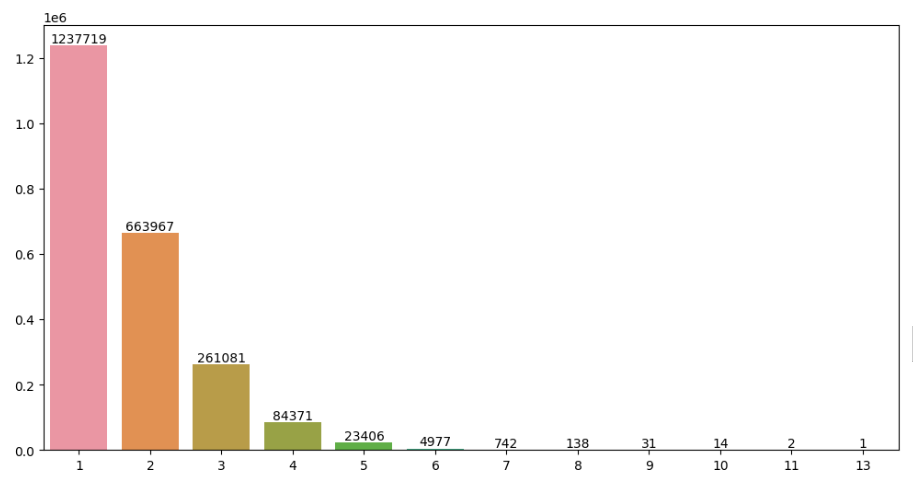
\includegraphics[scale = 0.5]{statistics/categories_count_plot.png}
    \caption{Categories Count Plot}
    \label{fig: Categories Count Plot}
\end{figure}




\section{Expected Outcome}
We expect to assign label to the new paper based on the title and abstract of the given paper using the multi label classifier model.

Using recommendation system, user should be able to get the similar paper for the given paper. 

